\begin{slide}
    \begin{block}{Lexical Analysis}
        Transform a list of characters found in the source file into a list of
        tokens defined in the language.
    \end{block}
    \vfill
    \begin{figure}[H]
        \centering
        \begin{tikzpicture}
            [node distance=1cm]
            \node[block] (input) {List of characters};
            \node[block,right=of input] (lexer) {Lexer};
            \node[block,right=of lexer] (output) {List of tokens};
            \draw[line] (input) -- (lexer);
            \draw[line] (lexer) -- (output);
        \end{tikzpicture}
        \caption{Lexical analysis overview}
        \label{fig:lexer_overview}
    \end{figure}
\end{slide}
\begin{slide}
    \begin{figure}[H]
        \centering
        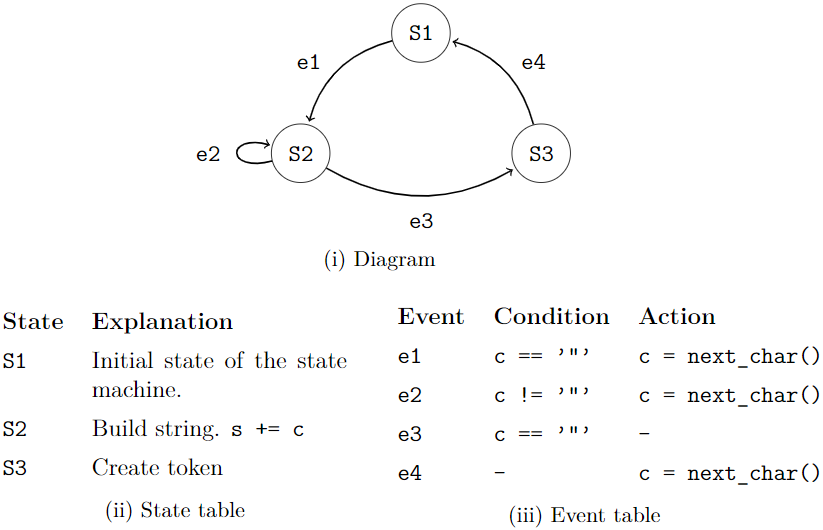
\includegraphics[width=0.9\textwidth]{finitestate}
        \caption{Example finite state machine for strings}
    \end{figure}
\end{slide}
\begin{slide}
    \begin{figure}[H]
        \centering
        \begin{tikzpicture}[node distance=1cm]
            % Nodes
            \node[square, minimum height=0.75cm, minimum width=1cm,] (n1) {...};
            \node[square, minimum height=0.75cm, minimum width=1cm, right of=n1] (n2) {\texttt{"}};
            \node[square, minimum height=0.75cm, minimum width=1cm, right of=n2] (n3) {\texttt{a}};
            \node[square, minimum height=0.75cm, minimum width=1cm, right of=n3] (n4) {\texttt{b}};
            \node[square, minimum height=0.75cm, minimum width=1cm, right of=n4] (n5) {\texttt{c}};
            \node[square, minimum height=0.75cm, minimum width=1cm, right of=n5] (n6) {\texttt{"}};
            \node[square, minimum height=0.75cm, minimum width=1cm, right of=n6] (n7) {...};
            % Lines
            \draw[line] ($(n2.south) + (0, -0.75)$) node[anchor=north] {\texttt{start\_ptr}} -- (n2);
            \draw[line] ($(n6.south) + (0, -0.75)$) node[anchor=north] {\texttt{current\_ptr}} -- (n6);
        \end{tikzpicture}
        \caption{Lexer scan technique}
        \label{fig:scanner}
    \end{figure}
    \begin{center}
        $\texttt{length} = \texttt{current\_ptr} - \texttt{start\_ptr} + 1$
    \end{center}
\end{slide}
\begin{slide}
    \begin{figure}[H]
        \centering
        \begin{tikzpicture}[node distance=1cm]
            % Nodes
            \node[square, minimum height=0.75cm, minimum width=1cm] (n1) {...};
            \node[square, minimum height=0.75cm, minimum width=1cm, right of=n1] (n2) {\texttt{w}};
            \node[square, minimum height=0.75cm, minimum width=1cm, right of=n2] (n3) {\texttt{h}};
            \node[square, minimum height=0.75cm, minimum width=1cm, right of=n3] (n4) {\texttt{i}};
            \node[square, minimum height=0.75cm, minimum width=1cm, right of=n4] (n5) {\texttt{l}};
            \node[square, minimum height=0.75cm, minimum width=1cm, right of=n5] (n6) {\texttt{e}};
            \node[square, minimum height=0.75cm, minimum width=1cm, right of=n6] (n7) {...};
            % Token nodes
            \node[square, anchor=west, minimum height=0.75cm] at ($(n1.south west) + (0, -2)$) (token) {\texttt{const char *start = \phantom{X}}};
            \node[square, minimum height=0.75cm, right = -0.025cm of token.east] (token1) {\texttt{const uint32\_t length = 5}};
            % Lines
            \draw[dot_arrow] ($(token.east) + (-0.2, -0.05)$) -- (n2.south);
        \end{tikzpicture}
        \caption{Token instance}
    \end{figure}
\end{slide}
